\chapter{Study Design}\label{chapter:studydesign}
The main goals of this thesis were to:
\begin{enumerate}
\item develop an exergame which can be used for warm up routine before more strenuous physical activity, and
\item evaluate its effectiveness in terms of guiding the user through the process of warming up.
\end{enumerate} In this chapter we outline the research framework, detail the research methods, and present the obtained results.
\section{Description of the Experiment}
This section describes the evaluation of the second version of the Immotion exergame. For this purpose, an approach was adopted that uses a mixture of different tools and user study methods. During this period, data has been logged, surveys have been conducted, and interviews undertaken. Similarly to the evaluation of the prototype exergame (Chapter 2), the obtained results are analyzed in order to determine to which level our proposed solution was effective in the given context and whether it offered a solution to the problem. %Based on the results from the exergame prototype evaluation (Chapter: Implementation) and a variety of research presented (Chapter Related Work), guidelines were followed which influenced the design and development of the second version of the Immotion exergame. 

\subsection{Introduction and Goals} \label{chapter:goals}
%II. AIMS
%The objectives of this research were to answer the
%following questions:
%A. How do sixth form students percieve gamification in CPR
%teaching?
%B. Does teaching CPR to sixth form students using direct
%feedback manikins change student’s attitudes towards:
%1) Confidence in performing CPR and use of an
%Automated External Defibrillator (AED)?
%2) Willingness to perform CPR and use an AED?
%3) Perceived competence in performing CPR and using an
%AED?
%C. Can we promote healthy living through CPR training?
%The overall aim of the project is to introduce students to
%CPR training using mobile uploads of scores, direct feedback
%via the CPR manikin and gamification through a competitive
%online leaderboard and increasing difficulty levels. The
%information gathered will help establish how best to use these
%techniques when teaching CPR in schools and will be used to
%set up a yearlong project in the schools to teach CPR.%

The first study evaluated the prototype exergame. Based on the results obtained, comments, and suggestions, the prototype exergame has been modified to better suit the needs of its future users. The primary goal of the second study was to investigate whether our exergame solution can be used as an interactive guide for individuals who do not know how to perform warm up routines. In addition, we examined if the exergame can be used as a solution that motivates individuals to warm up before physically more demanding exercises, and provides an enjoyable game experience. Taking this into account, the research questions we address in this study are as follows: 
\begin{enumerate}
\item \textbf{RQ1: Evaluation of effectiveness} - How effective our proposed solution is in guiding the user through the warm up routine compared to the guidance offered by classic (traditional) methods?
%\item Comparing the experience between participants that use the exergame and participants that do not use the exergame. 
%\item Can our proposed solution motivate individuals to undertake warm up procedure?
\item \textbf{RQ2: Evaluation of perceived usefulness and ease of use} - How useful and easy to use our proposed solution is?
\item \textbf{RQ3: Evaluation of the usability} - How usable our proposed solution is? 
\item \textbf{RQ4: Evaluation of the game experience} - How enjoyable and entertaining our proposed solution is? 
\end{enumerate}
%The actual warm up was the original procedure:  
%\begin{itemize}
%\item The warm up routine was derived from sports literature.
%\item The exergame has been designed with this in mind.
%\item A video has been recorded with the original procedure.
%\end{itemize}http://edutechwiki.unige.ch/en/Usability_and_user_experience_surveys
%http://www.nigelbevan.com/papers/What_is_the_difference_between_usability_and_user_experience_evaluation_methods.pdf
In order to evaluate the effectiveness, perceived user experience, usefulness and usability of our gamified solution in the given context, the user base is divided into two groups: \textit{experiment group} and \textit{control group}. The first, experiment group, is the one that interacts with the exergame directly. Contrarily, the control group is presented with the video of a coach (professional) who guides the participant through the warm up routine. This division allows us to infer the influence of our gamified solution, as well as, to assess the main differences in completing the required activities between the two user groups. 
%\subsubsection{Assumptions}
%\begin{itemize}
%\item The participants will be able to perform the requested movements.
%\item The participants will answer all the questionnaires truthfully.
%\item The software and hardware that is used used will function properly.
%\end{itemize}
\subsubsection{Hypotheses}
%Remember to state these in terms of the independent and dependent variables. If it is not immediately clear why you would have a certain hypothesis (it often follows logically from the introduction of the experiment), then include a brief explanation separate from but following the hypothesis. You do not need to state the null hypothesis.%
Based on the research questions outlined in the previous section, the following hypotheses are established to be tested: 
\begin{enumerate}
\item \begin{math}H_{1}\end{math}: The exergame itself is sufficient for guiding the player through a proper warm up procedure with correct movements. 
\item \begin{math}H_{2}\end{math}: After the warm up routine is completed using the exergame, player's ROM is increased.
%\item Participants that are interactively guided through the warm up procedure using the exergame have perceived exertion during physical activityexertion during a testperceived user experience in terms of PRC scale, compared to the participants who warm up without the exergame.
\item \begin{math}H_{3}\end{math}: Participants had a more positive perceived warm up experience when using the exergame compared to the participants not using the exergame.  
%\item Participants can easily follow the exergame and perform all the required movements. MODIFY %felt more motivated to undertake warm up exercises when using the exergame compared to the participants not using the exergame.
%\item The exergame will encourage more 
%behavior change compared to the standard warm up %procedure. - for longer study
\end{enumerate}
\pagebreak
%Introduce your experiment, and give the reader the specific goals you expect it to address. It is common at this stage to give the reader a hint of your hypotheses (if they are not already hinted at in the Introduction).%
\subsubsection{Apparatus}
The experiment was conducted in the laboratory room in DFKI. The laboratory is presented in Figure \ref{fig:lab1}.\\ 
\begin{figure}[h]
    \centering
    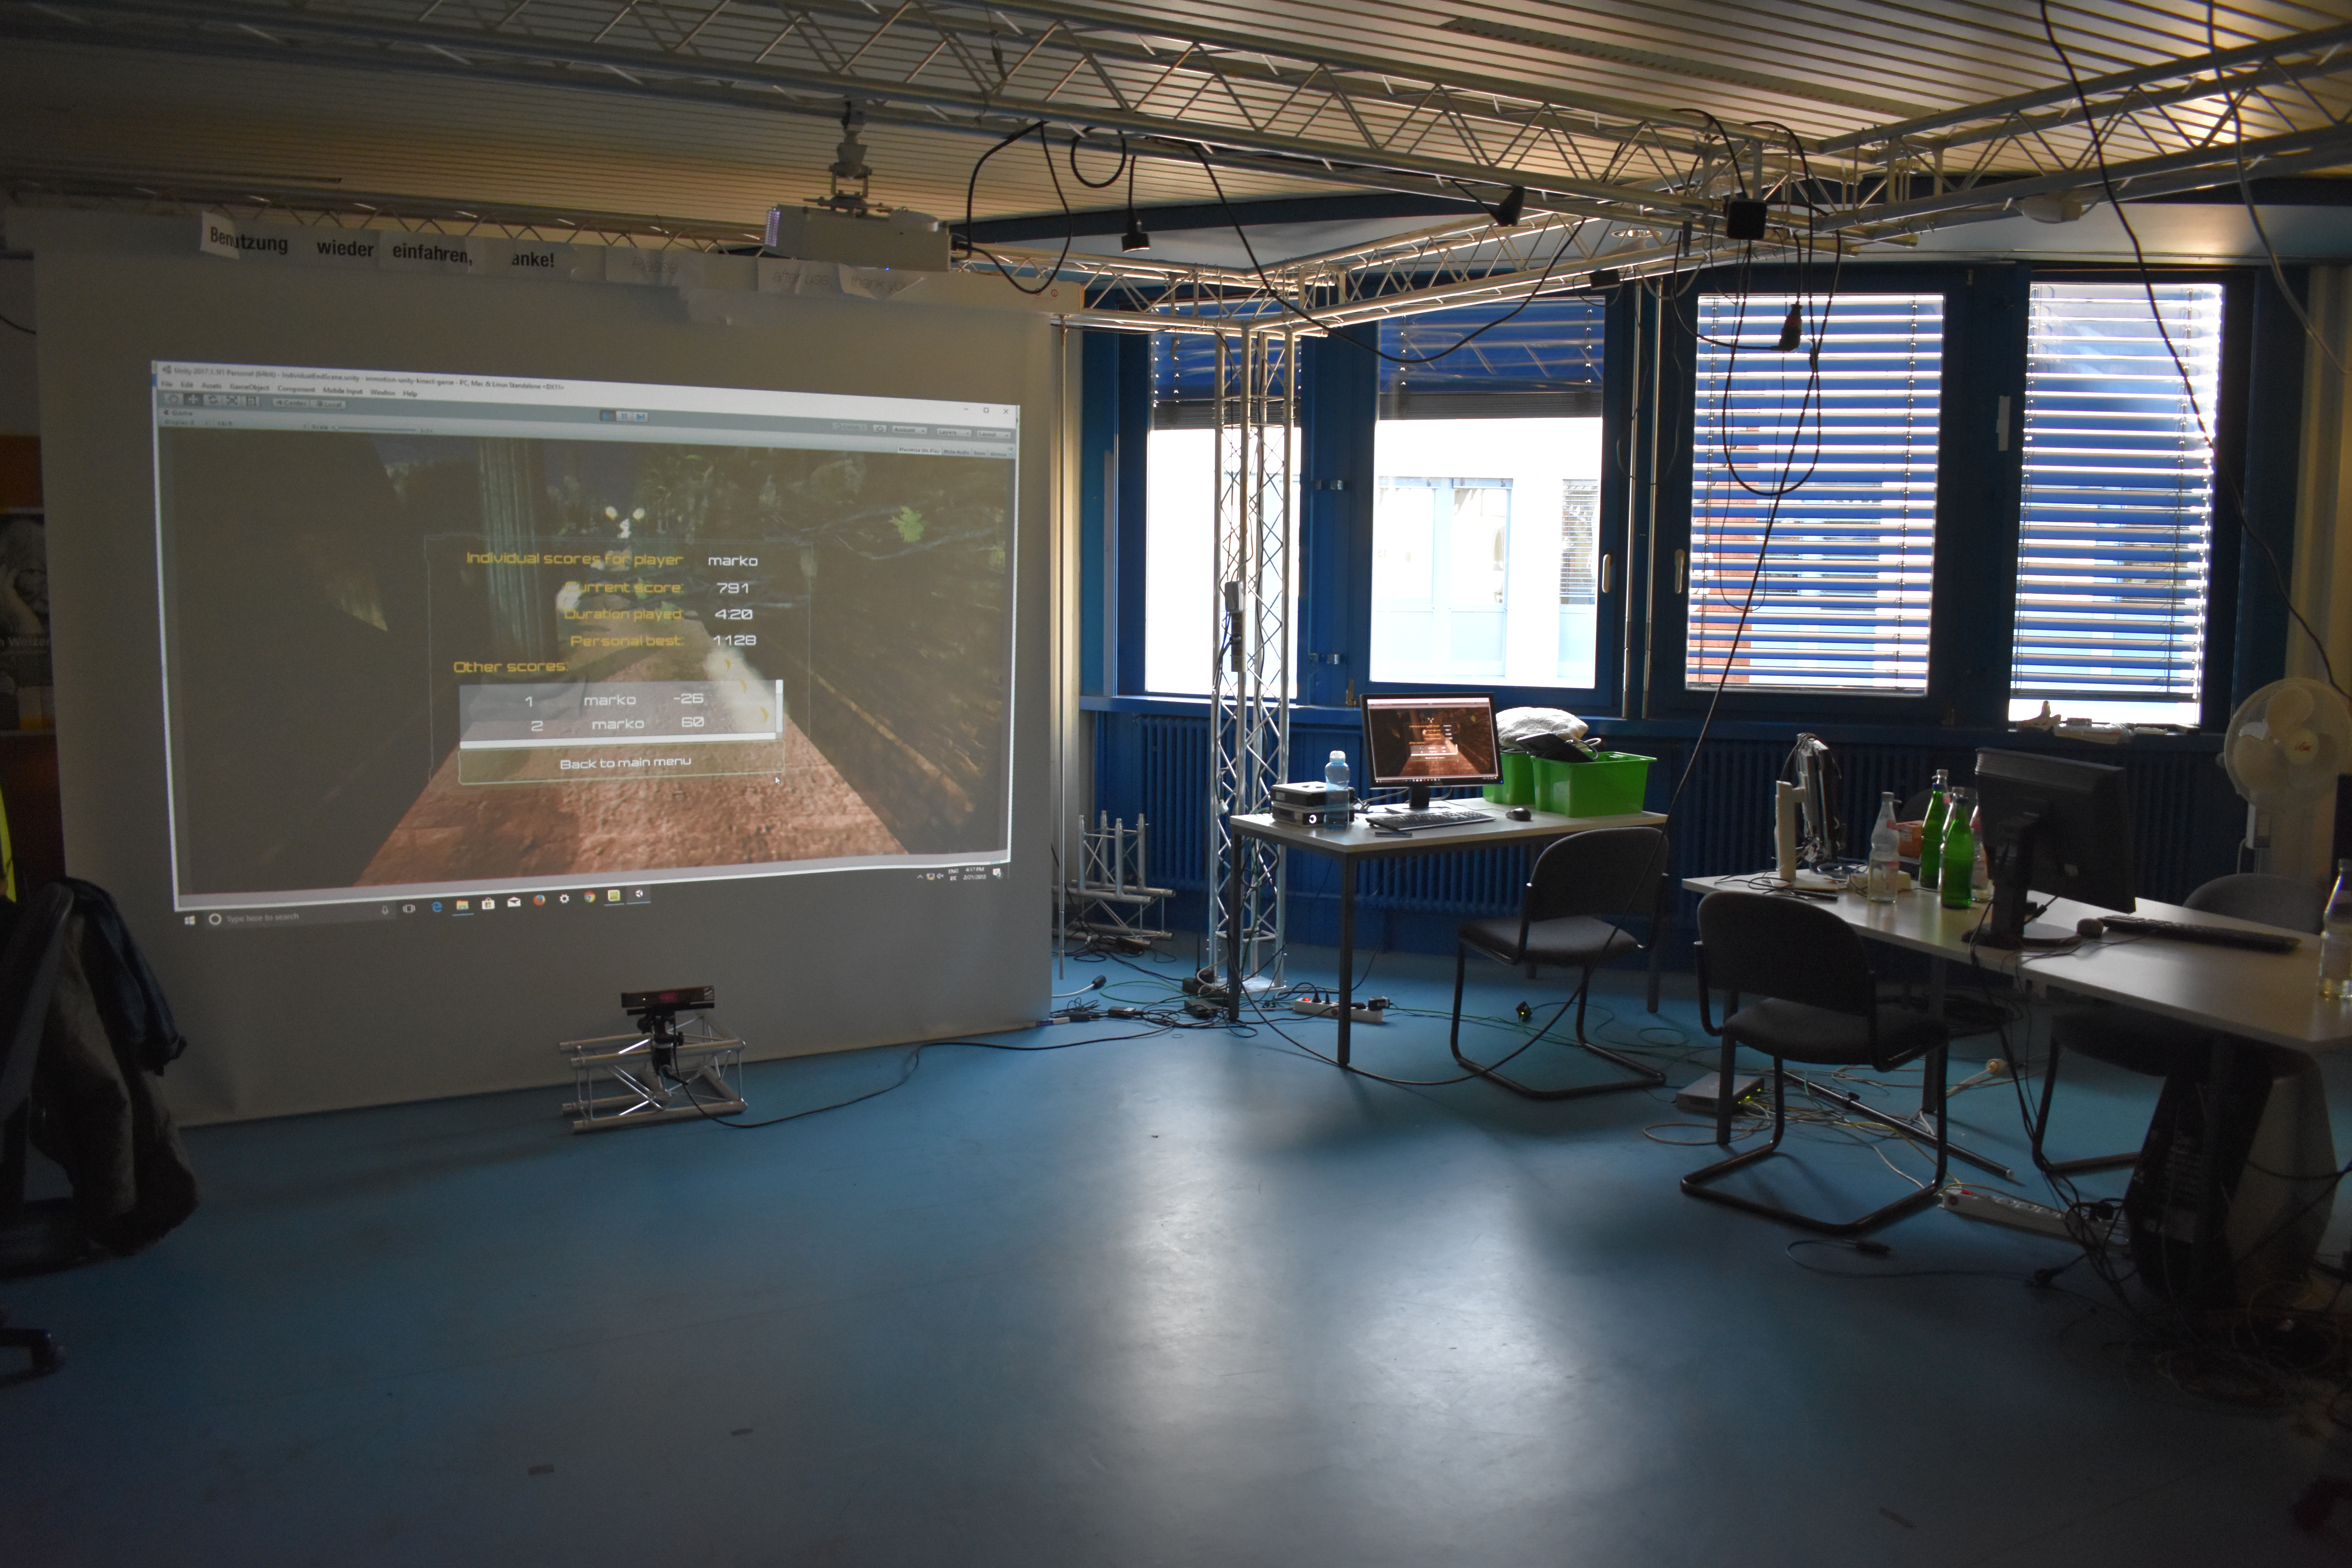
\includegraphics[width=0.9\textwidth]{Room1}
    \caption{Laboratory.}
    \label{fig:lab1}
\end{figure}\\
The following equipment has been used during the experiment:
\begin{itemize}
\item Kinect for Xbox One (2.0 2013) motion sensing input devices by Microsoft used for movement detection and controlling the exergame avatar. 
\item Kinect for Xbox One (2.0 2013) motion sensing input devices by Microsoft used for recording the experiment. 
\item PC running the game engine.
\item Projector used to display the game (video) on the wall in front of the participant.
\item Microsoft Band used for gathering skin resistance data.
\item Polar H7 Bluetooth Heart Rate Sensor and Fitness Tracker for hear rate and respiratory rate monitoring.
\item Camera for taking photos of participants' facial expressions during the warm up procedure.
\item Goniometer used for measuring participants' \acrshort{rom}.
\end{itemize}\pagebreak
Both the Kinect motion sensors have been placed in front of the display panel facing the participant playing the exergame. The participant was instructed to keep at least 2 meter distance from the sensor during the gameplay. This distance was the most optimal in order for the system to function properly in terms of skeleton tracking. The sensor is presented in Figure \ref{fig:kinect}.\\
\begin{figure}[h]
    \centering
    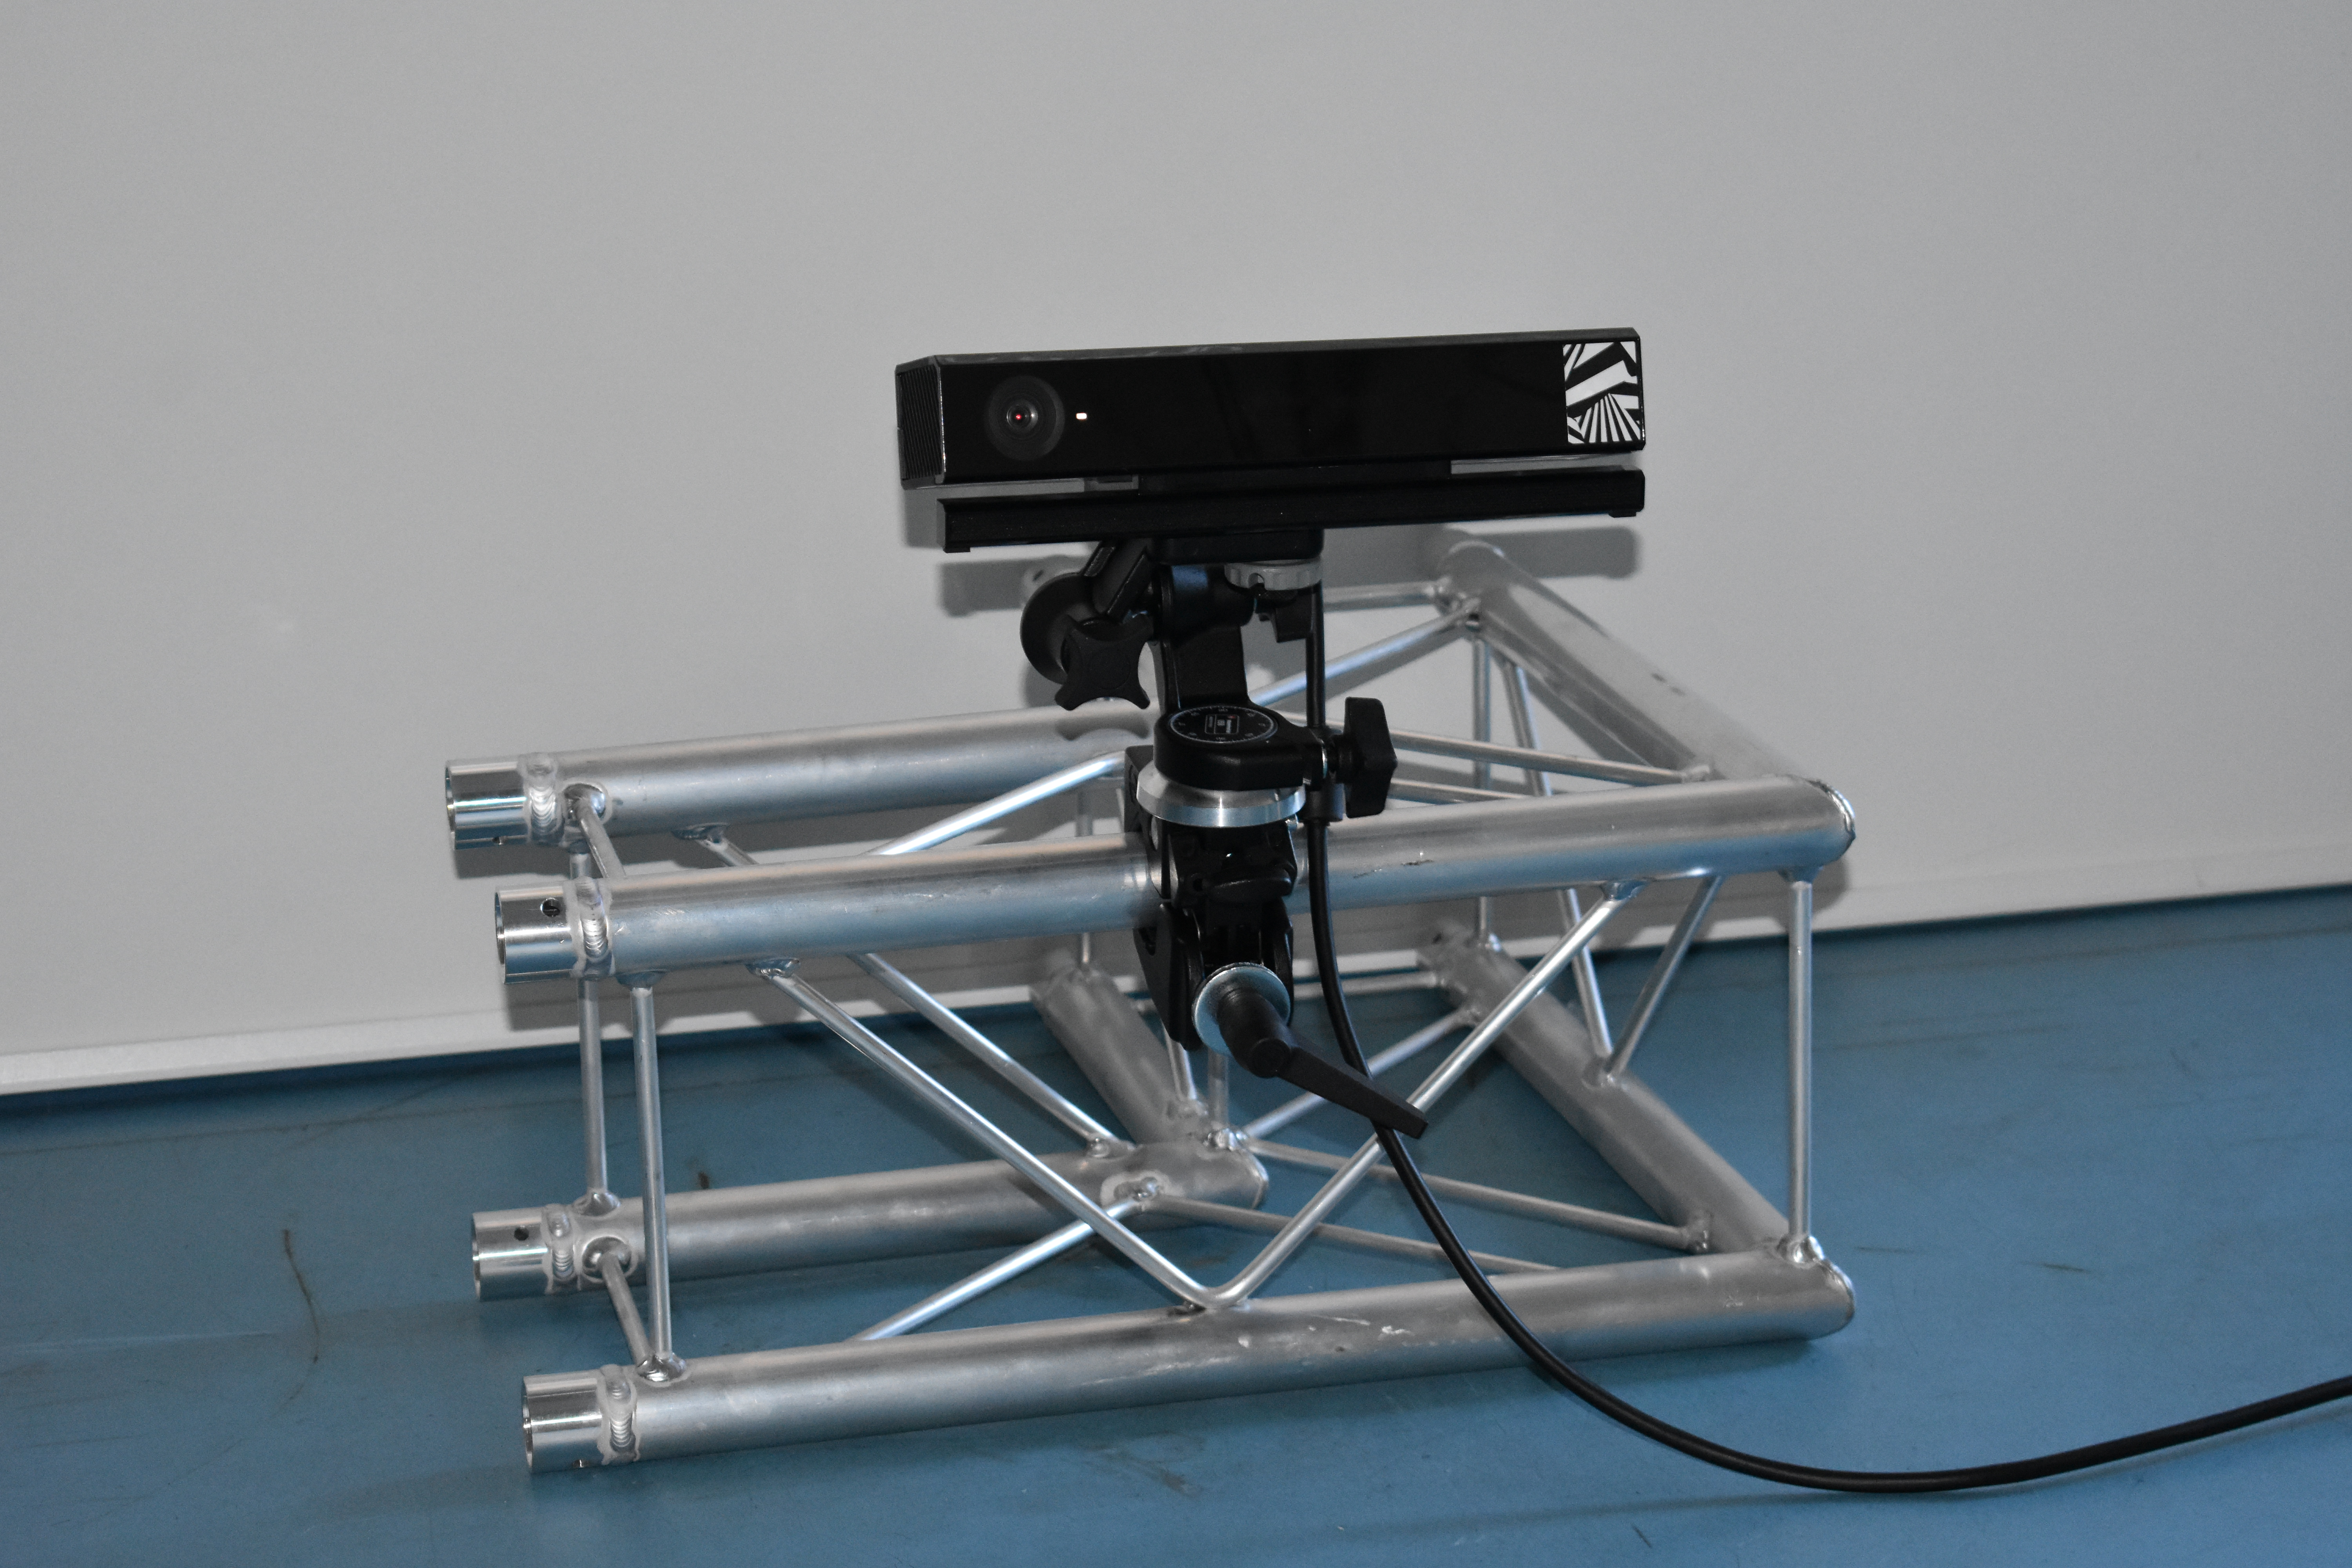
\includegraphics[width=0.9\textwidth]{Kinect}
    \caption{Kinect motion sensor.}
    \label{fig:kinect}
\end{figure}\\
We used a projector in order to display the exergame and video to the participants that was placed above the user so it did not interfere with the game flow. The desktop set up is presented in Figure \ref{fig:desktop}.\\
\begin{figure}[h]
    \centering
    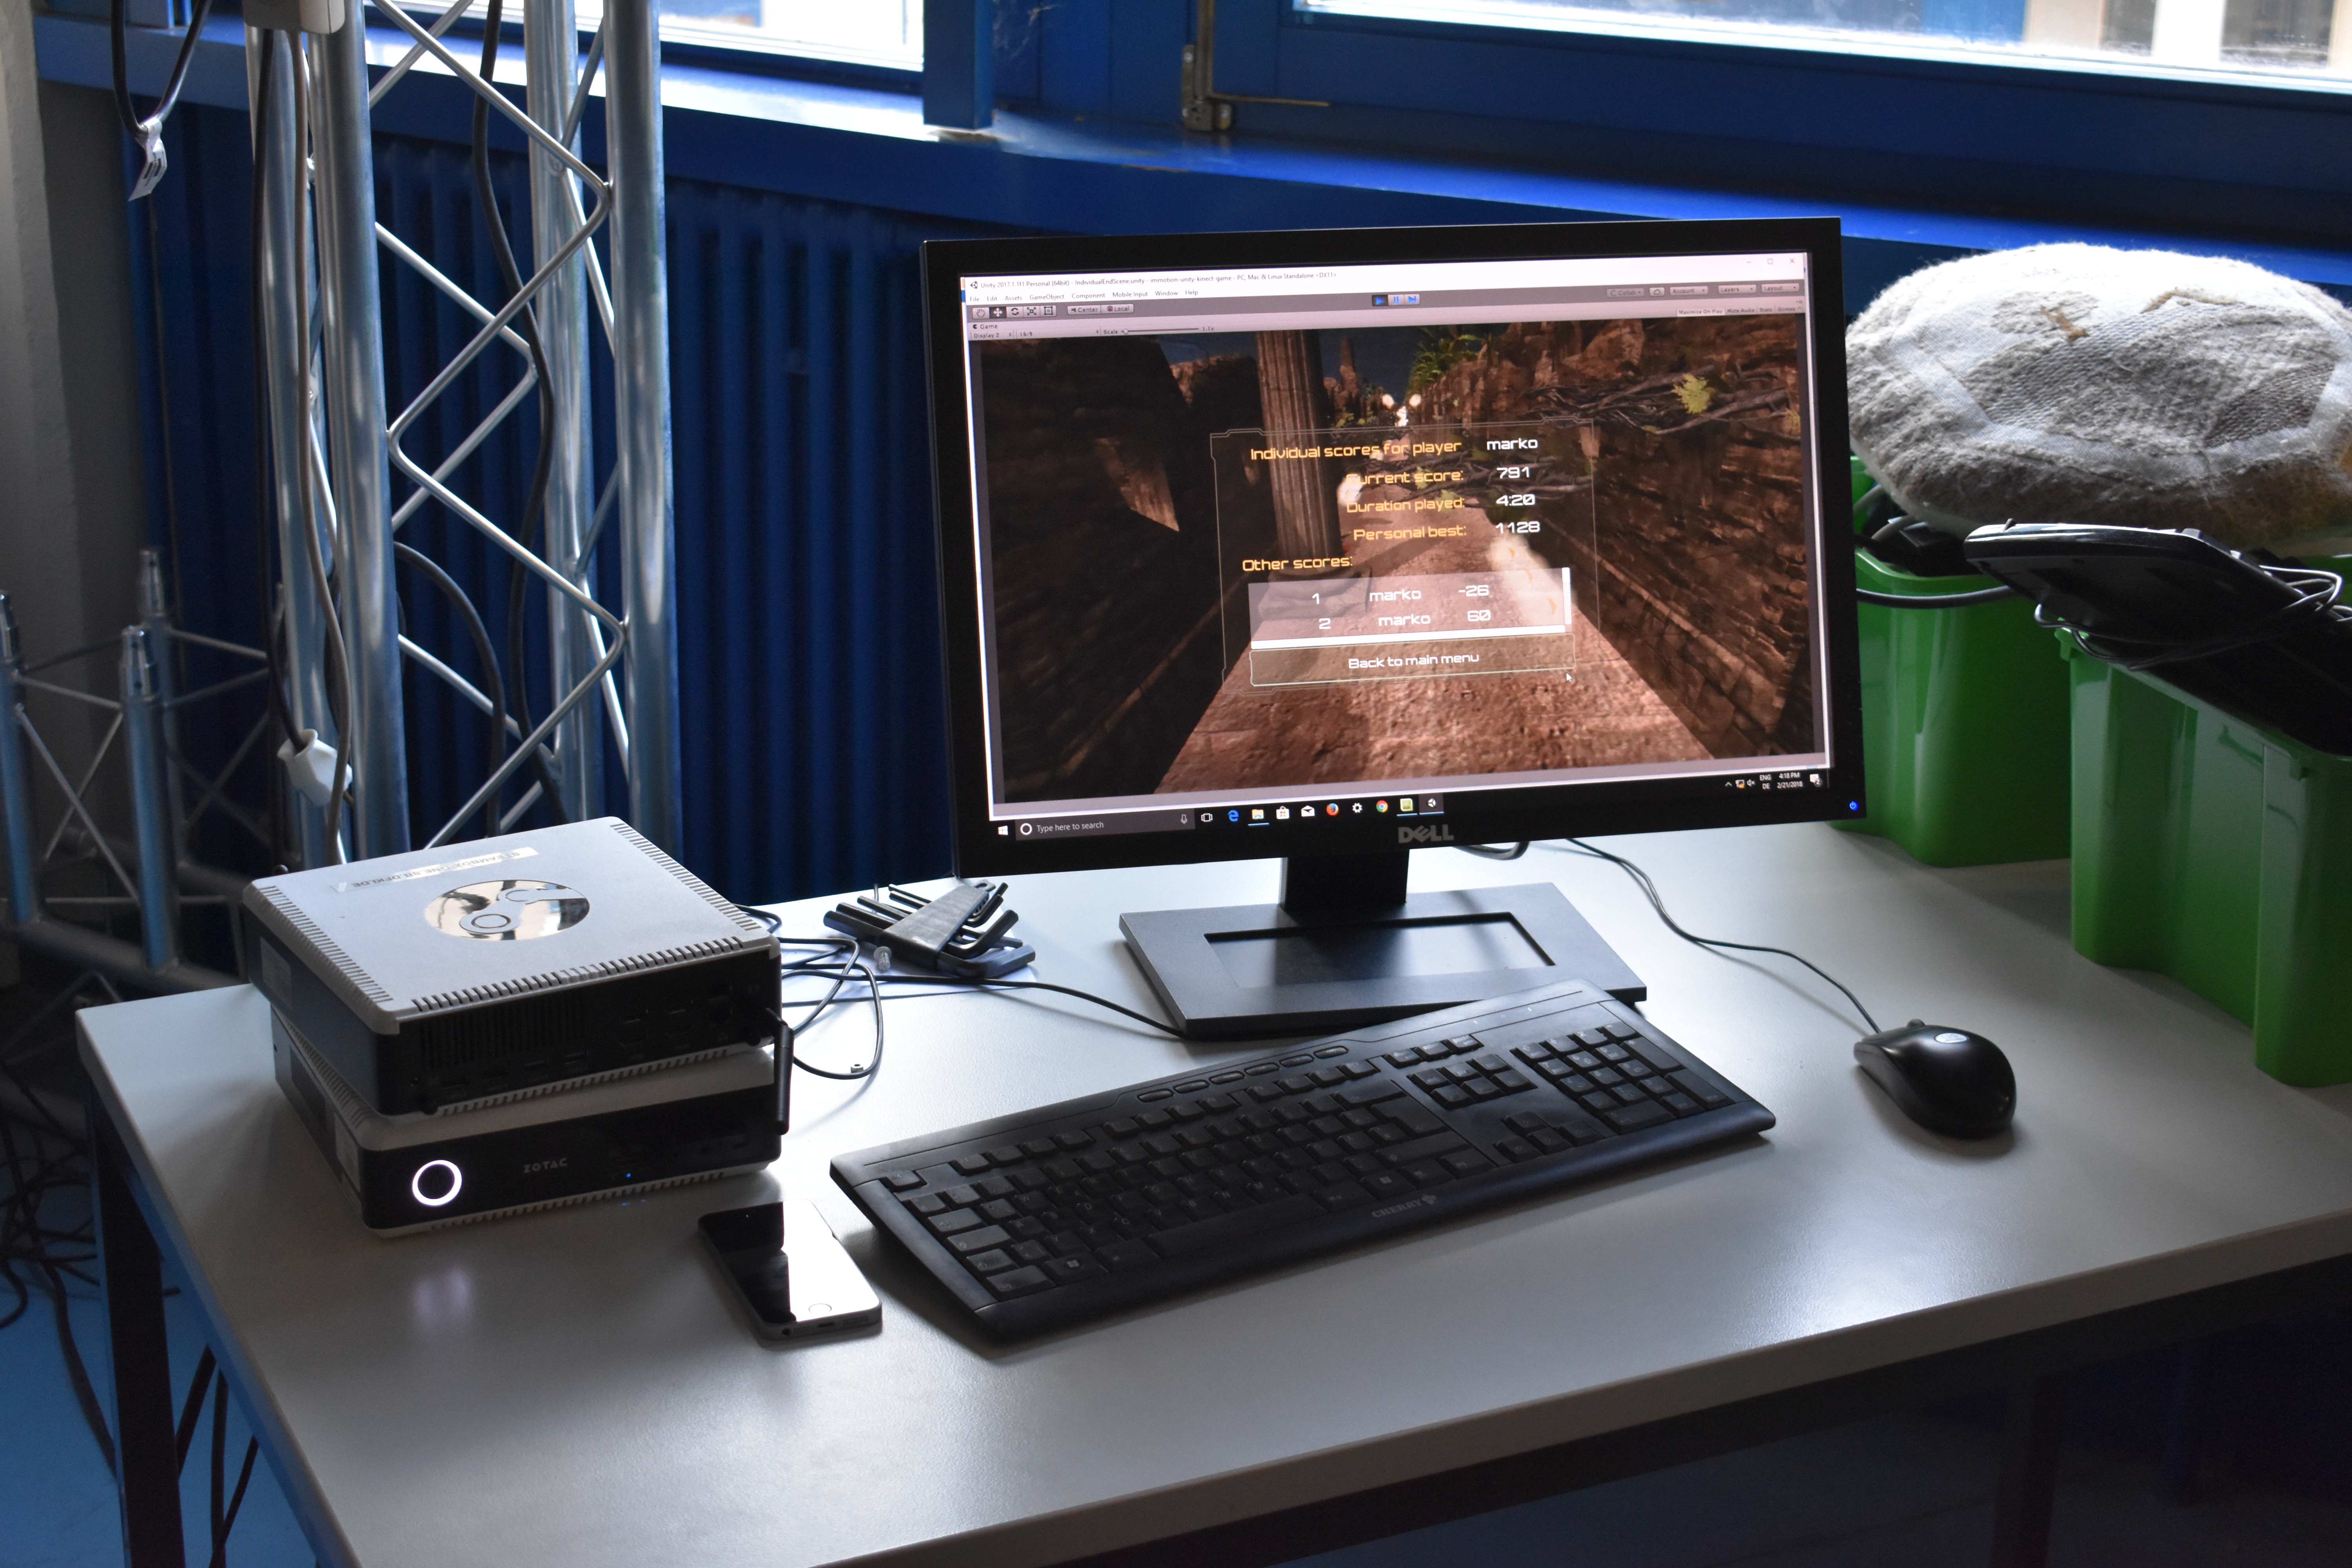
\includegraphics[width=0.9\textwidth]{Desktop}
    \caption{Desktop set up.}
    \label{fig:desktop}
\end{figure}
%\begin{figure}[h]
%    \centering
%    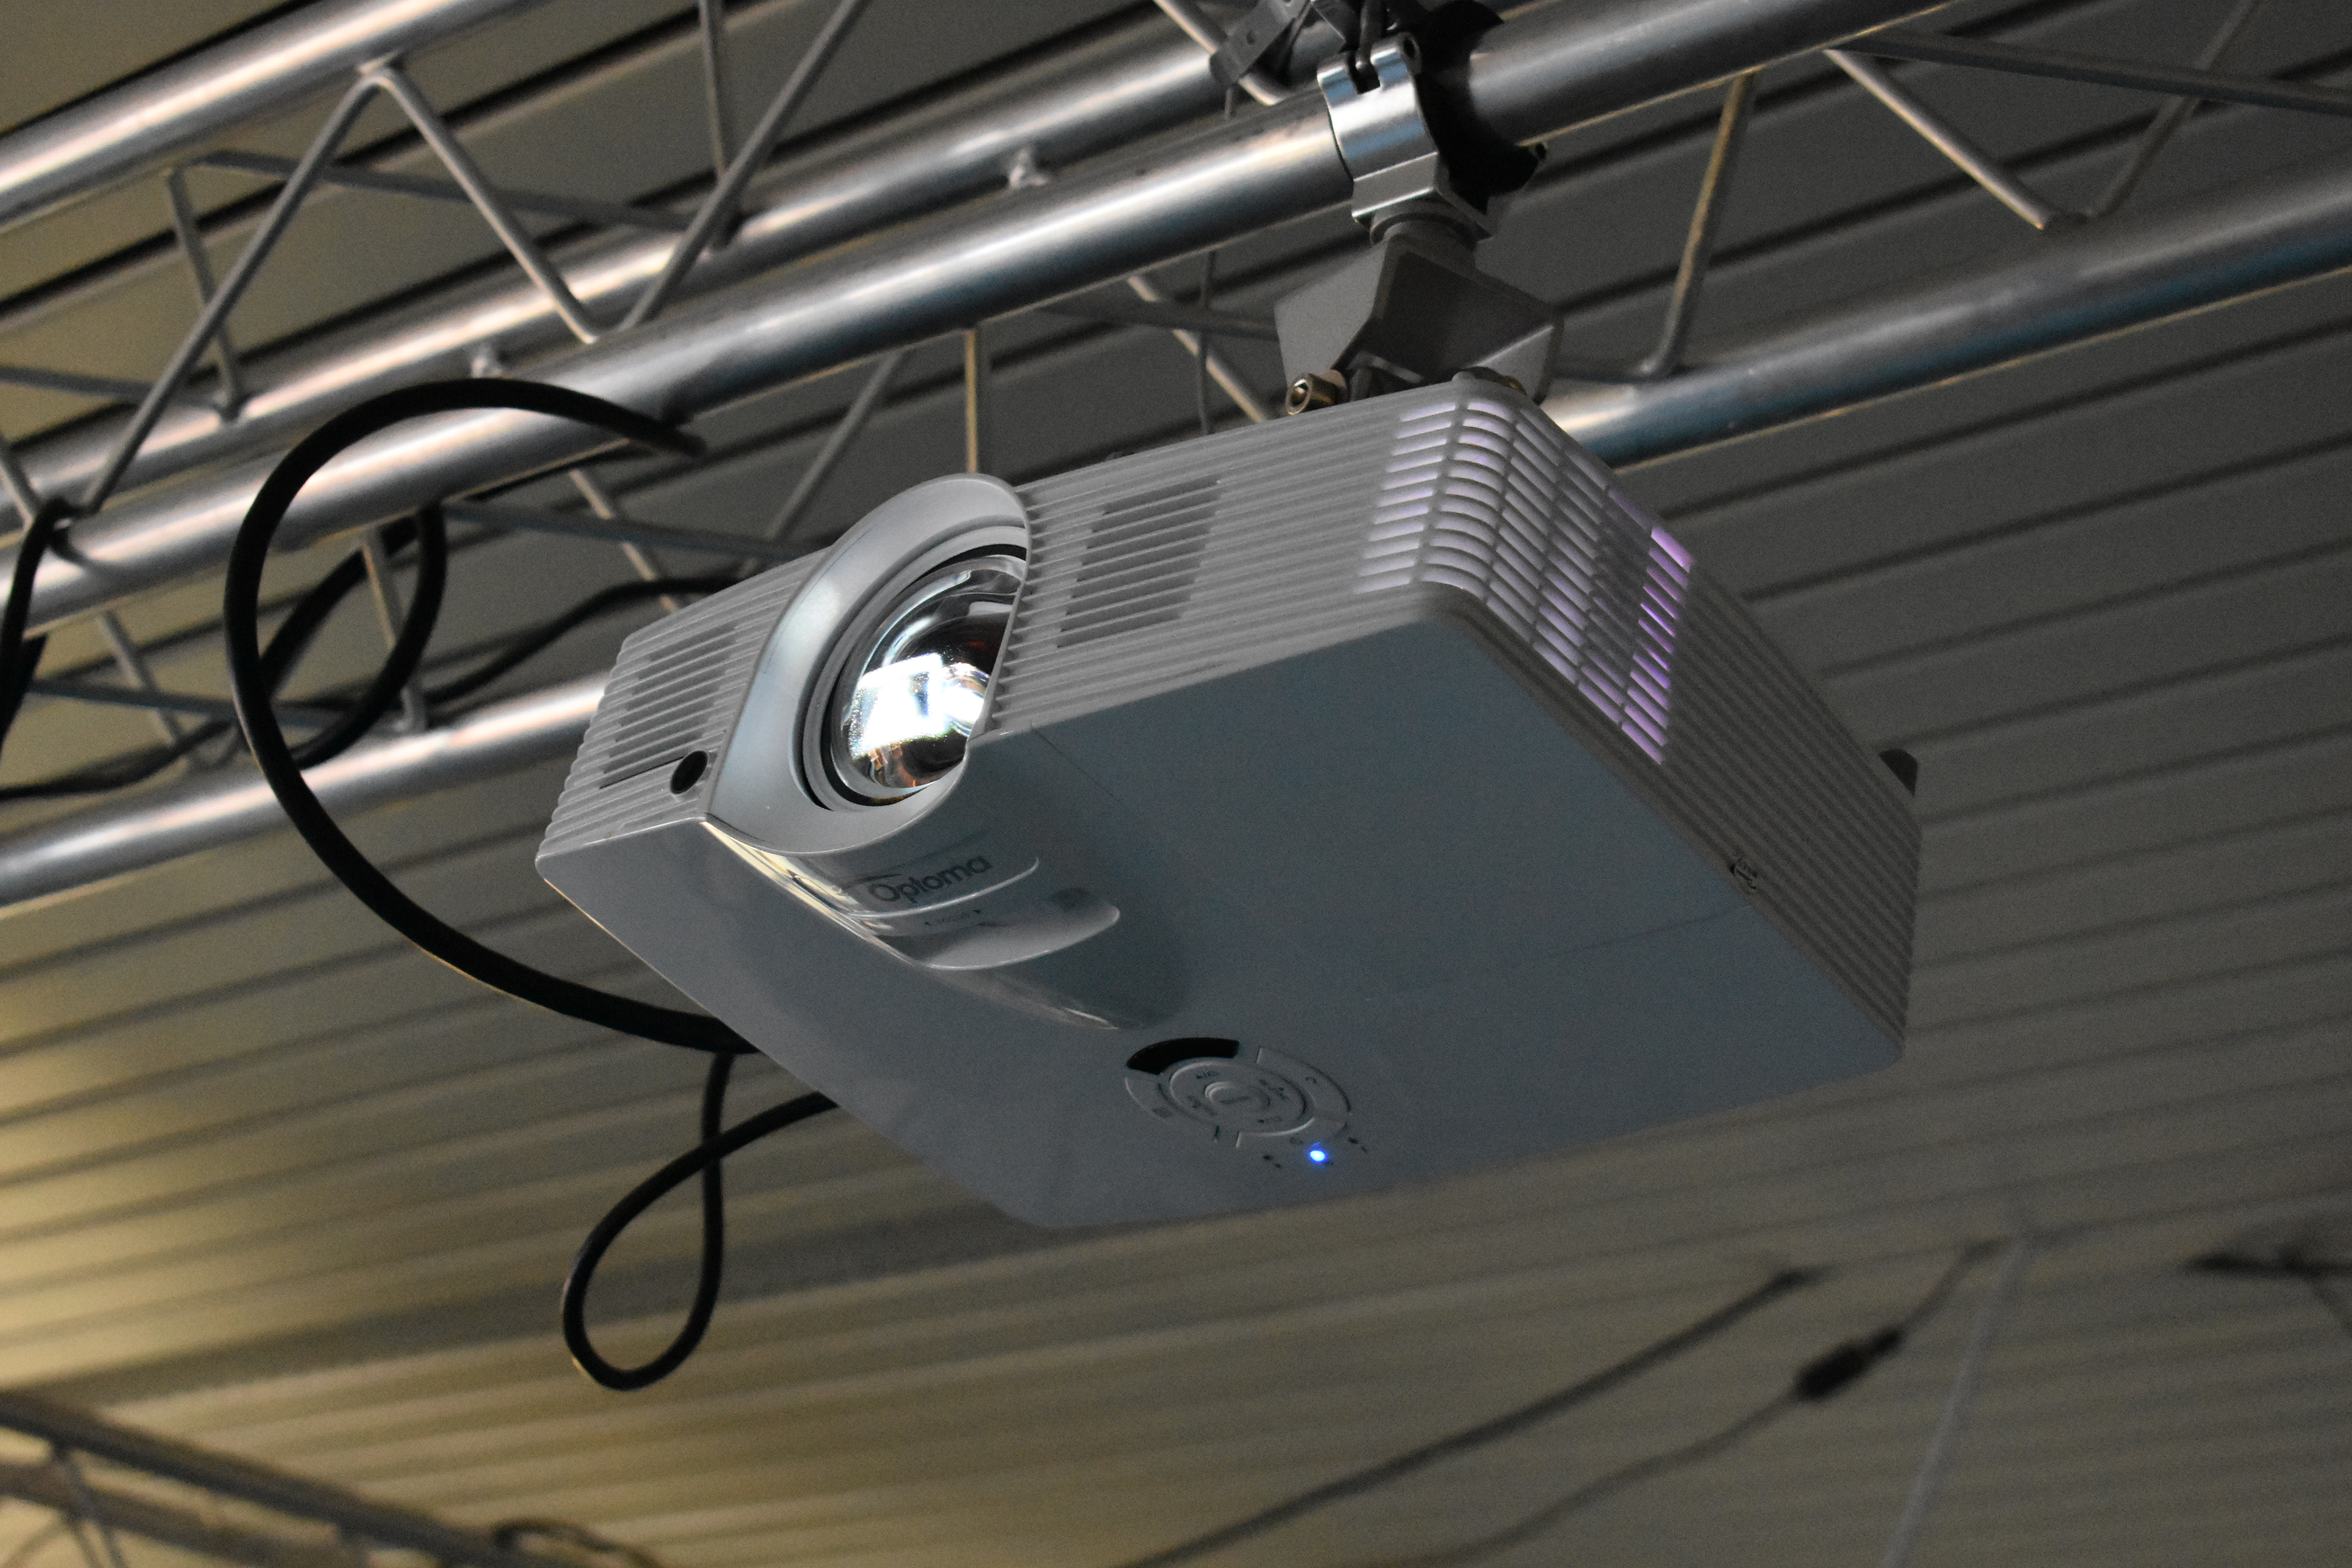
\includegraphics[width=0.9\textwidth]{Projector}
 %   \caption{Projector.}
 %   \label{fig:projector}
%\end{figure}
\subsection{Methods} 
In this section we outline the methodology adopted for the Immotion exergame evaluation. For this purpose we utilize the traditional (moderated) usability test since it gives direct input on how real users use the system. %First, we measure users' performance. That is, we measure the time users' will spend performing the warm up exercises with the exergame and with the video. The amount of time users' feel warmed up sufficiently. 
%We decide to follow a mixed-methods approach, and by doing so, utilize both qualitative and quantitative data sources in combination. Second, we measure users' satisfaction level. What the user thinks about his interaction with the product (visually appealing) 
%
%This is a detailed description of the experiment that should allow other researchers (familiar with HCI and experimental design in general, but not familiar with your experiment) to replicate your experiment.%
\subsubsection{Participants}
The study has been conducted on \displaydate{date1} and \displaydate{date2} in DFKI. All participants were students from Saarland University. All the participants reported no physical impairment at the time of participating in the study. For recruiting participants, posters were distributed in print, and sent through social media and email (Appendix X). Each participant was given 10 euros cash for taking part in the study. All of the participants were amateur athletes who engage in some physical activity on average 4 times per week. For the study we particularly targeted individuals who exercise in gym or fitness centers and often avoid preforming warm up exercises before more strenuous physical activity. All participants were required to report to the laboratory in gym based clothing, preferably shorts and t-shirt, and all of them performed the required tests in the same location using the same equipment. Before the study, each participant signed a consent form (Appendix X).%Describe your participants (e.g., any relevant demographics, if/how they were divided into categories), including total number, and recruiting approach. Indicate if any incentives were used. Comment on the representativeness of your participants relative to the target population, if their representativeness isn’t immediately obvious.%
\subsubsection{Conditions}
First 10 participant who applied for the experiment have been accepted. These participants were sent a pre-test questionnaires (\acrshort{bsa}, \acrshort{parq}, and a Demographic questionnaire) that needed to be completed before coming to the experiment. Based on the answers given, the participants were assigned to the control or the experiment group. Each assigned participant took part in a single test session one hour in duration. During this session, all the participants  performed one warm up session, after which they completed a set of questionnaires. Two conditions were evaluated:
\begin{enumerate}
\item Warming up with the exergame guiding through the warm up procedure, projected on a wall in front of the participant.
\item Warming up with a video of a professional (coach) guiding through the exact same warm up procedure as induced by the exergame, projected on a wall in front of the participant.
\end{enumerate}
Depending on the group, each participant performed exercise that represent one of the conditions.
\subsubsection{Control and Experiment Groups}
The participants were assigned to each group based on the previously completed self-reported questionnaires. These questionnaires were sent to each participant and needed to be completed before the experiment. Based on the answers provided, each participant was assigned to either control or experiment group. The surveys assessed participants' perceived physical fitness level, warm up preferences, and previous exergames experience.
\subsubsection{Measures and Metrics}
%All tasks were performed under a cognitive walkthrough approach, and all data was
%recorder. After performing the tasks, and taking the CUE-model [12] as a framework and
%following adaptations already mentioned in literature review (cf. ([13]; [14];[15]; [16]), three
%instruments were used in order to assess the users’ perspectives about the applications’
%instrumental and non-instrumental qualities, and the user’s emotional reactions to the whole
%experience.
%For assessing the applications’ instrumental qualities (e.g. controllability, effectiveness,
%learnability), the research team used the SUS - System %Usability Scale [17] and the
%Pragmatic dimension of AttrakDiff [18]. The SUS-scale [17] is %a 10-item questionnaire with a
%5-point Likert scale developed to assess several usability aspects such as ease of use and
%usefulness. As for AttrakDiff [18], it is an instrument created to measure the attractiveness of
%an application by presenting the user/evaluator three groups of opposite adjectives.
%AttrakDiff records both the perceived pragmatic quality, the hedonic quality and the
%attractiveness of an interactive product or application.
%For accessing non-instrumental qualities (e.g. aesthetics, identification) the research team
%used the AttrakDiff Hedonic dimension.
%Finally, for the evaluation of emotional reactions (e.g. valence, arousal, control of the
%application), the research team used the SAM - Self-assessment Manikin [19]. The
%SAM-Manikin is a non-verbal pictorial assessment method that directly assesses the
%pleasure, arousal, and dominance associated with the user’s affective reactions to a certain stimuli.
%Qualitative data was also collected through a semi-structured interview conducted at the end
%of the test session, aiming to get the participant’s opinion regarding the application (its main
%features), the interface and the adopted solutions
Two separate sets of questionnaires were administered, one
prior to the experiment session and one post the session in order to gather self-reported user perception data.
The pre-test questionnaires focused on participants' demographic information, overall physical and psychological abilities, hours spent on exercise, frequency and activity
of warm up procedures, extent of video gameplay, and reason for playing. The pre-test questionnaires were as follows:
\begin{itemize}
%https://www.researchgate.net/publication/320572645_Exergaming_Feels_good_despite_working_harder

\item \textit{Health status}. The current health status of the participants has been assessed via the \gls{parq}, which consists of seven dichotomous items \cite{thomas1992revision}. The individual response patterns were used in order to assess if participants were physically able to perform the warm up session.
\item Demographic survey with included questions regarding warm up preferences, and previous exergame experience [Appendix].
\item \textit{Physical activity screening}. Pre-study physical activity levels have been assessed with a standardized questionnaire  \gls{bsa} \cite{fuchs2015messung}. Participants were instructed to indicate for how many minutes per week they performed everyday physical activities (e.g., taking the bike to work; taking a walk) in average during the last four weeks. 
\end{itemize}
The second set of questionnaires have been administered after the completion of the warm up procedure. In these questionnaires participants' level of exertion, emotional state, and game experience have been assessed. The questionnaires were as follows:
\begin{itemize}
\item \textit{Perceived exertion}. For assessing the perceived exertion of the warm up session, the \gls{rpe} has been utilized \cite{borg1998borg}. The perceived exertion reflects how difficult and strenuous the performed warm up exercise feels to the participants, combining all sensations and feelings of physical stress, effort, and fatigue.
\item \textit{Emotional state}. The pleasure, arousal, and dominance associated with a person's affective reaction to a wide variety of stimuli has been assessed with \gls{sam} \cite{bradley1994measuring}. 
\item \textit{Enjoyment of the physical activity}. To test the enjoyment of the physical activity performed, in this case the warm up procedure, the \gls{paces} has been used \cite{kendzierski1991physical}. 
\item \textit{System usability}. For assessing the exergame's instrumental qualities (e.g. controllability, effectiveness, learnability), the \gls{sus} has been used.
\item \textit{Enjoyment of the play}. In order to measure the play enjoyment and experience o the \gls{pes} has been utilized \cite{pavlas2012play}. 
\end{itemize}
During the experiment, the following metrics were collected from each participants:
\begin{itemize}
\item \textit{Range of motion}. The participants' \acrshort{rom} has been measured before and after the warm up routine using goniometer.
\item \textit{Heart rate and Respiratory rate}. The participant's heart rate data has been captured and the measured during the warm up procedure using Microsoft Band.
\item \textit{Distance}. The overall distance the participants' moved during the warm up routine was measured using Microsoft Kinect. 
\item \textit{Skin resistance}. TODO
\item \textit{Participant's emotion}. TODO
\end{itemize}
The warm up routine performed by the participant has been recorded using a second Kinect sensor for further analysis of performed movements during the warm up procedure.
%If your experiment is comparing multiple different interfaces or interactive systems or techniques, describe each of them. Screen snapshots of interfaces/systems are particularly useful.%
\subsubsection{Tasks}
In order to interact with the gamified system, the participants in the experiment group were required to perform a set of general movements. By performing these movements, the participant controlled the game avatar and, by doing so, attempted to avoid obstacles and collected coins. Based on the data and feedback gathered from the first study, we limited the movements the participants needed to perform in the exergame. That is, only movements that are detectable with high accuracy using only one Kinect device and simplistic enough to be accomplished easily without no prior exercise knowledge or experience were required to be executed by the participants. These movements were: 
\begin{itemize}
\item right hand movement up,
\item left hand movement up,
\item jump right,
\item jump left,
\item jump up, 
\item star jump, and
\item squat.
\end{itemize}
Participants who were in the control group and did not interact with the gamified system were required to perform the same set of general movements. However, participants in this group had to follow a video and not interact with the exergame. The video was a recording of a professional (coach) who guided the participants through the warm up routine. By following the video, and thus the coach, the participants were required to execute the same movements in the same order as the participants in the experiment group who interacted with the exergame.
%Briefly describe what participants were asked to do with the interactive system(s).%
\subsubsection{Procedure}
The study protocol was reviewed and approved by an institutional ethics committee. For data collection, we used a  paper and pencil as well as \textit{Google forms} questionnaires. Before the experiment, the lab environment was set up. The Kinect sensor was placed in a correct position and turned on. The PC running the software was started and the projector is enabled. In each session only one participant was present and guided by the researcher.\\\\\\\\\ The activities each participant followed were:
\begin{itemize}
\item The participant completes the preliminary survey.
\item The researcher explains the sensors and tools that are required for the experiment, after which the participant puts them on. 
\item After the researcher confirms that the sensors are placed in a correct position, we start recording heart rate data.
\item The researcher measures the participant's \acrshort{rom} before starting the warm up procedure. The following \acrshort{rom}'s are assessed: 
\begin{itemize}
\item Left and right shoulder rotation
\item Left and right shoulder extension
\item Left and right hip flexion
\item Left and right hip extension
\end{itemize}
\item After the measurements are collected, the participant rests while the researcher explains what is required from the participant.
\item The researcher gives a general explanation on the benefits of a proper warm up routine before physically more demanding exercise.
\item The participant moves to the spot marked by the researcher.
\item The researcher starts recording the session. 
\item The warm up procedure begins:
\begin{itemize}
\item If this participant is part of the experiment condition, the game begins with the \textit{Start scene}. The researcher inputs the participant's name and presses the \textit{Start} button. After 5 seconds, the game proceeds with scenes in which the participant is required to perform specific movements in order to avoid obstacles and collect coins. The duration of the game is not fixed and it is played up to the point when the participant feels warmed up enough. 
\item  In case the participant is part of the control group, the video that displays a coach who instructs the participants which movements need to be performed. As with with the sessions in the experiment group, the duration of the warm up is not fixed and the video is played up to the point when the participant feels warmed up enough.
\end{itemize}
\item After finishing with the warm up routine, the participant takes a rest. The data collection is stopped. During this period the sensors are removed from the participant. \item Researcher assesses the \acrshort{rom}  of the participant. 
\item The participant completes the post-test surveys . %https://www.verywell.com/rating-of-perceived-exertion-scale-3119445
\end{itemize}
%\subsubsection{Independent and Dependent Variables}
%Include exactly how you intend to measure each dependent variable. 
%https://books.google.de/books?hl=de&lr=&id=bPhLeMBLEkAC&oi=fnd&pg=PP1&dq=measuring+the+user+experience&ots=R9KdcqS-vF&sig=2-V-FaMOeX24Rn0pG30lWVdvjSo#v=onepage&q=measuring%20the%20user%20experience&f=false
%Independent variables are the things you manipulate or control for, such as design's you are testing or the ages of the respondents. 
%Dependent variables are the things you measure, such as success rate, number of errors, user satisfaction, completion time, and many more. Have s clear idea what do you manipulate - independent variables, and what do you want to measure - dependent variables. The most interesting is the intersection - is one design results in a higher task success rate than other. Independent and dependent variables can be measured by 4 types of data: nominal, ordinal, interval, and ratio. 
%Nominal (categorical) data: groups or categories. Mac vs Windows users, male vs female. These are independent variables, that allows you to segment data by these different groups. Nominal data also includes dependent variables like task success, number of users who clicked link A instead B... 
%Ordinal: ordered data - imdb. In user studies this comes from self-reported data. User states if someone is good better worse... These are relative rankings. You report it by frequencies: for example 40 percent said it is good. 

\subsection{Problems/Limitations - Threats to Validity}
Our participant sample has an unbalanced gender ratio and a limited age range, which represent a limitation for the study results. Moreover, the arms of the standard goniometer that has been used for measuring participants' \acrshort{rom} were not longer than 12-inches which made it difficult to accurately pinpoint the exact landmark needed for measurement.
\section{Results}
Our subject group included 10 individuals, of which 2 were female and 8 were male. Participants were on average age \begin{math}\bar{x} = 26.7\end{math} years old (\begin{math}SD= 1.77,  x_{max}=30 ,x_{min}= 24 \end{math}), with different levels of education, such as Bachelor's degree (n = 4) and Master's degree (n = 6). Two participants reported to exercise 7 to 8 times per week and only 1 participant 5 to 6 times per week. The majority of the participants exercise 1 to 2 times (n = 3) or 3 to 4 times (n = 4) per week. The duration of the sport or fitness activity for most of the participants was between 1 and 2 hours long (n = 8). Only 2 participants reported engaging in sports activity with duration less than 1 hour. The most common exercises the participants reported doing during one fitness or sport session were:
\begin{itemize}
\item Anaerobic exercise - sit-ups, pull-ups, push-ups, squats, and weight lifting (n = 8).
\item Team sports - football, basketball, cricket, handball, etc (n = 4).
\item Running outdoors, running on treadmills, and doing yoga (n = 3).
\item Cycling and jogging (n = 2).
\end{itemize}
The majority of the participants (n = 7) engage in physical activity alone, while only 3 participants enjoy sports activities performed in a group. TODO. Out of 10 participants, 4 reported not engaging in warm up exercises before sports sessions. The most common reasons reported by the respondents were time constraint (n = ), the monotonous and tiresome nature of the warm up procedure(n = ), how the warm up procedure represents an insignificant and negligible activity (n = ), and lastly, that no one warms up either (n = ). Regarding duration of the warm up session, 6 participants reported spending less than 5 minutes for warming up, while 4 participants reported spending between 5 and 10 minutes on this preparatory activity.\\
\begin{figure}[h]
    \centering
    \includegraphics[width=0.9\textwidth]{participantExperiment}
    \caption{Participants during the experiment performing the worm up procedure.}
    \label{fig:participants}
\end{figure}\\
%\begin{figure}[h]
 %   \centering
%    \includegraphics[width=\textwidth]{GameTypes}
  %  \caption{Game types most often played by the participants.}
    %\label{fig:gametypes}
%\end{figure}\\
Out of all the participants, 7 stated that they engage in sport specific warm up, whereas 3 reported engaging in general  (non-specific) warm up exercises. Half of the participants (n = 5) stated that they do not enjoy warming up in a group. When inquired about preferences regarding warming up when given instruction, 6 participants stated they prefer warming up when given instructions, while 4 participants stated they do not prefer warming up when given instructions. The engagement in playing video games varies among the participants: 1 plays video games daily, 1 few times per month, 1 once per month, 2 once a day, 3 few times per year, and 4 once per year or less. The most common game types among participants are racing (n = 5) and sports games (n = 4). In addition, when inquired about participant's previous experience with Microsoft Kinect games, only 1 participant reported having a lot of experience with games in this area. The rest of the participants reported having either non or some experience with Kinect related games.\pagebreak

\subsection{Range of Motion}
\gls{rom} has been assessed  for each condition before the warm up session and immediately the participants completed the procedure. For taking the measures a plastic goniometer with 1 degree increments has been utilized. The average \acrshort{rom} values for each condition are presented in Figure \ref{fig:romExperiment} and Figure \ref{fig:romControl}.
\begin{figure}[h]
    \centering
    \includegraphics[width=\textwidth]{ROMSummaryExperiment}
    \caption{Summary of ROM results for the experiment group.}
    \label{fig:romExperiment}
\end{figure}
\begin{figure}[h]
    \centering
    \includegraphics[width=\textwidth]{ROMSummaryControl}
    \caption{Summary of ROM results for the control group.}
    \label{fig:romControl}
\end{figure}\\
We observe that the average values after the warm up session for all measured joints are higher in each experiment condition. These increased measures imply that our exergame solution, as traditional warm up procedures, positively affects one's \acrshort{rom}.
\subsection{Warm Up Duration}
The duration of the warm up session has been measured from the game or video start until the moment the participant stopped with the warm up session. The participants have been informed to play the game or follow the video instructions as long as they usually spend on warm up session before some physically strenuous activity. The average warm up duration for the experiment condition was \begin{math}\bar{x} = 800.4 \end{math} seconds (\begin{math} SD = 205.4, x_{max}=1122, x_{min}=616 \end{math}). The average warm up duration for the control condition was \begin{math}\bar{x} = 444.2 \end{math} seconds (\begin{math} SD = 94.2, x_{max}= 576, x_{min}= 345\end{math}). The average duration with standard error of the warm up session for each conditions is presented in Figure \ref{fig:wuduration}. The average duration of the warm up session for the participants in the experiment group who played the exergame is significantly higher compared to the duration of the warm up session for the participants in the control group. That is, interacting with the exergame positively influenced the duration of the warm up session for all the participants in the experiment condition.\\
\begin{figure}[h]
    \centering
    \includegraphics[width=0.9\textwidth]{AVGTime}
    \caption{Average WU duration with standard errors per study group.}
    \label{fig:wuduration}
\end{figure}\\
An independent-samples t-test was conducted to compare average warm up duration in experiment and control conditions. There was a significant difference in the scores for experiment (M=, SD=) and control (M=, SD=) conditions; t (8)=2.89, p = 0.20. These results suggest that the our exergame does have an effect on warm up duration. That is, our results suggest that when warm up duration increases significantly when performed using our exergame. 
\subsection{Heart Rate}
The heart rate data has been captured and monitored using Polar H7 Bluetooth Heart Rate Sensor and Fitness Tracker in order to determine the exercise intensity of a warm up session. The heart rate has been measured from the beginning of the warm up session until the moment the participant declared being warmed up enough for a subsequent hypothetical physical activity. The average maximum heart rate for the participants in the experiment group was \begin{math}\bar{x} = 174.20 \end{math} (\begin{math} SD= 7.01, x_{max}=186, x_{min}=170 \end{math}). The average maximum heart rate for the participants in the control group was \begin{math}\bar{x} = 158.8 \end{math} (\begin{math} SD= 10.06, x_{max}= 169, x_{min}= 144\end{math}). Figure \ref{fig:hrdata} presents the average heart rates with standard errors per condition. From the figure is evident that the participants in the experiment condition reached higher heart rate levels compared to the participants in the control condition.\\ %The exergame was more successful in placing more participants in their target heart rate range and in the target heart range for cardio-respiratory benefits.
\begin{figure}[h]
    \centering
    \includegraphics[width=0.9\textwidth]{AVGHr}
    \caption{Average heart rate per study group.}
    \label{fig:hrdata}
\end{figure}\\
The individual heart rate data for each participant is depicted in Figure \ref{fig:hrCumulative}. It can be observed, as previously pointed out, that the participants in the experiment group who interacted with the exergame solution, reached higher level of heart rates during the warm up session compared to the participants in the control condition. Furthermore, from the figure is evident that the duration of the warm up session for the participants in the experiment group is significantly longer also.\pagebreak
\begin{figure}[h]
    \centering
    \includegraphics[width=\textwidth]{HRCumulative}
    \caption{Heart rate data for each participant. The color represents the condition the participant belongs to.}
    \label{fig:hrCumulative}
\end{figure}\\
For each participant we calculated the zone of the target heart rate (\begin{math} T_{HR}\end{math}) based on the maximum heart rate using the Karvonen method. A number of formulas are used to estimate  \begin{math} HR_{max}\end{math} [wiki]. Tanaka, Monahan, \& Seals (2001) proposed the following formula for calculating \begin{math}HR_{max}\end{math}\\
\begin{equation}
THR_{max} = 208-(0.7 * age)
\end{equation}The resting heart rate \begin{math} R_{HR}\end{math} have not been measured during the experiment session. Hence, we utilized the generalized values for \begin{math} R_{HR}\end{math} based on age groups []. Since our participant engage in sports activities sami-regularly, we opted for the \textit{average} generalized \begin{math} R_{HR}\end{math} values. The heart rate reserve (\begin{math} HS_{R}\end{math}) represents the difference between participant's heart rate at rest and heart rate at maximum effort, and has been calculated as follows: \begin{equation}
HR_{R} = THR_{max} - R_{HR} 
\end{equation}The Target minimum heart rate (\begin{math} THR_{min}\end{math}) has been calculated for each participant using the following formula:\begin{equation}
THR_{min} =  HR_{R}*0.5 + R_{HR} 
\end{equation}
Following, the Target moderate heart rate (\begin{math} THR_{mod}\end{math}) has been calculated as follows:\begin{equation}
THR_{mod} =  HR_{R}*0.7 + R_{HR} 
\end{equation}Lastly, the Intense target heart rate (\begin{math} THR_{int}\end{math}), to be reached during extreme-intensity anaerobic exercise, is calculated as follows: 
\begin{equation}
THR_{int} =  HR_{R}*0.85 + R_{HR} 
\end{equation} If the participant's heart rate falls into the middle of the (\begin{math} T_{HR}\end{math}) range, that means the participant is exercising at moderate intensity (roughly 50 to 70\% of \begin{math} THR_{max}\end{math}). In case it verges toward the upper limit, the participant is exercising at high intensity (70 to 85\% of \begin{math} THR_{max}\end{math}). Figure \ref{fig:hrZones} presents the calculated target zones for the participants.\\
\begin{figure}[h]
    \centering
    \includegraphics[width=\textwidth]{HRTargetZones}
    \caption{Computed target zones for participants in each condition.}
    \label{fig:hrZones}
\end{figure}\\
It can be observed that the maximum heart rates of the participants in the experiment group obtained during the warm up fall in the middle and lower range of high intensity exercise. Only one participant's (ID = 4) heart rate was close to the maximum target heart rate (\begin{math} THR_{max}\end{math}). On the other hand, the maximum heart rate of the participants' in the control group fall in lower range of high intensity exercise with one participant (ID = 7) in the middle range of moderate intensity exercise zone. Figure \ref{fig:hrzones} depicts the distribution of maximum heart rates participants reached during warm up session in both condition per exercise intensity zones. Figure \ref{fig:hrzones} depicts three distinct zones (\textit{Low, Moderate, and High} intensity zones) that were computed based on participants' age, resting heart rate, and heart rate reserve (Figure \ref{fig:hrZones}). The figure gives a clearer overview of the intensity of the warm up performed in both condition. It can be observed that the participant in the experiment group reached higher levels of exertions compared to the participants in the control group. This can be attributed to the duration differences between the conditions.\pagebreak
\begin{figure}[h]
    \centering
    \includegraphics[width=\textwidth]{HRZonesPic}
    \caption{Target heart rate with exercise intensity for each participant}
    \label{fig:hrzones}
\end{figure}\\
%In general, participants reached the target minimum heart rate relatively promptly. 
Overall, we conclude that  participants in both conditions reach an elevated heart rate sufficient to continue with the more strenuous physical activity. The results, however, suggest that the duration  of the warm up session for the participants in the experiment group can be shortened in order to keep the heart rates at moderate levels. 
%Lastly, we compared the times participants in the experiment and control conditions reached target minimum and moderate heart rate. Figure \ref{fig:hRTargetMinMod} depicts the differences between the conditions.\\ 
%\begin{figure}[h]
 %   \centering
  %  \includegraphics[width=0.9\textwidth]{HRTargetMinMod}
%    \caption{Minimum and moderate target HR.}
 %   \label{fig:hRTargetMinMod}
%\end{figure}\\
I%t can be observed that the participants in the control group have reached both target heart rate much faster than the participants in the experiment group.\pagebreak

%\subsection{RR data}
%The average RR data per condition is presented in Figure \ref{fig:rrdata}.
%\begin{figure}[h]
  %  \centering
   % \includegraphics[width=0.9\textwidth]{AVGRr}
   % \caption{Average RR per study group.}
   % \label{fig:rrdata}
%\end{figure}\pagebreak
\subsection{Physical Activity Enjoyment Scale}
Given the benefits of physical activity and WU procedures, we needed to better understand how participants 
perceive physical activity participation. The \acrfull{paces} test consists of 18 questions in a 1 to 7 Likert scale that was originally designed to measure positive affect associated with involvement in physical activities in college students (Kendzierski and DeCarlo, 1991).  The high scores obtained on the positive items and low scores on the negative items indicate a high enjoyment of the physical activity. Whereas, the total enjoyment score is obtained by reversing negative item scores and summing them to positive item scores. We coded participants' responses, where higher scores indicated greater enjoyment, with scores ranging from 18 to 126. The participants in both conditions completed the \gls{paces} after finishing with the WU session. Figure \ref{fig:pacees} presents the average results for each question per condition. It shows that the participants in the experiment condition rated consistently higher all the questions with respect to the scores of the participants in the control condition. \\The questionnaire with all the questions can be found in Appendix X.\\
\begin{figure}[h]
    \centering
    \includegraphics[width=0.9\textwidth]{PacesSummary}
    \caption{Summary of PACES results for control and experiment group.}
    \label{fig:pacees}
\end{figure}\\
Figure \ref{fig:pacesPerCondition} depicts the average scores for all questions per condition. It can be observed that the average score for the control condition is \begin{math}\bar{x} = 89.8 \end{math} (\begin{math} SD = 11.97, x_{max}= 104, x_{min}= 71\end{math}), which is already high, but for the experiment condition is even higher  \begin{math}\bar{x} = 114.4 \end{math} (\begin{math} SD = 5.98, x_{max}= 125, x_{min}= 111\end{math}).\\
\begin{figure}[h]
    \centering
    \includegraphics[width=\textwidth]{pacesPerCondition}
    \caption{Average PACES scores for control and experiment condition.}
\label{fig:pacesPerCondition}
\end{figure}\\
After performing a normality test on the scores, we compared the the mean of the experiment (M = 114.40 , SD = 5.98) and control (M = 89.80 , SD = 11,97) group with a paired t-test (\begin{math}\alpha = 0.05\end{math})  we found a significant difference; t(8) = 4.11144, p = .003384. Whereas Conen's d was 2.594795. Therefore, we conclude that there is a difference between the two conditions and that warming up by using the exergame positively affects the physical activity enjoyment.
%Some of the things you may do here are: report means and standard deviations in neat tables indicate the statistics used and levels of significance include graphs, plots, histograms, etc that tell a story about the actual figures obtained Only critical raw data and summary statistics should be included in the actual report. However, you must keep all your raw data in a separate archival report, should anyone (a reviewer in the case of real scientific reporting) need more detail than is provided in the paper. 
\subsection{System Usability Scale}
The \acrfull{sus} is a reliable tool for measuring the usability of a system under tests. It consists of a 10 item questionnaire with five response options for respondents from strongly agree to strongly disagree. The sum of the 10 items in the questionnaire leads to a general measure of perceived usability of the system. The participants' scores for each question are converted, added together and then multiplied by 2.5 to convert the original scores of 0-40 to 0-100. Even though the scores are 0-100, these are not percentages and should be considered only in terms of their percentile ranking. Based on research, a  \acrshort{sus} score above a 68 would be considered above average and anything below 68 is below average. Only the participants in the experiment condition took the \acrshort{sus} questionnaire. The summary of the \acrshort{sus} scores is presented in Figure \ref{fig:sus}. It can be observed that the participants who interacted with the exergame gave the exergame relatively high scores. The  average \acrshort{sus} score for our exergame  is \begin{math}\bar{x} = 76.7 \end{math} (\begin{math} SD = 8.16, x_{max}= 90, x_{min}= 72.5\end{math}). This implies that our system usability received \textit{excelent} adjective rating and a \textit{B} on a grade scale \cite{brooke2013sus}.\\
\begin{figure}[h]
    \centering
    \includegraphics[width=\textwidth]{SUSSummary}
    \caption{Summary of SUS results per participant.}
    \label{fig:sus}
\end{figure}\\\\
The \acrshort{sus} average scores per question is depicted in Figure \ref{fig:susPerQuestion}. It can be observed that the participants found that the various functions in the exergame have been well integrated and that they felt very confident using the exergame. Furthermore, all the participants agreed that people would learn to use the exergame very quickly. Also, they did not find the exergame unnecessarily complex or having any unconsistencies during gameplay. They also thought that it was not difficult or awkward to use, and that getting familiar with the game was pretty straightforward and fast. When asked if they would like to continue playing the game frequently, 3 participants agreed with this statement, 1  neither agreed nor disagreed, and 1 disagreed. \\
\begin{figure}[h]
    \centering
    \includegraphics[width=\textwidth]{SUSPerQuestion}
    \caption{Summary of average SUS results for each question.}
    \label{fig:susPerQuestion}
\end{figure}
\subsection{Play Experience Scale}
The \acrfull{pes} is a valid and reliable 16 item questionnaire with five response options for respondents from strongly agree to strongly disagree \cite{pavlas2012play}. It has been utilized in order to assess play experience, usability, and enjoyment of our exergame. The \gls{pes} scale collects responses across four experiential dimensions which are labeled: \begin{itemize}
\item Freedom - when individuals are free in a play context, they are able to perform the actions they wish to perform.
\item No extrinsic - addresses if the respondents feel there are consequences to their play.
\item Play direct - addresses the play itself.
\item Autotelic/Focus - when experience is autotelic, an individual engages in it solely for its own rewards. That is, the experience is intrinsically motivating.  Focus targets the states of immersion and concentration during play. It is related to engagement and flow and the items in this category  reflects on the loss of concern and focused concentration.
\end{itemize}
Figure \ref{fig:pesPerQuestion} summarizes the PES results per question for each dimension discussed.\\
\begin{figure}[h]
    \centering
    \includegraphics[width=\textwidth]{PESSummaryPerQuestion}
    \caption{Summary of average PES score for each question. Yellow bars have been reverse-coded.}
    \label{fig:pesPerQuestion}
\end{figure}\\
In general, the participants enjoyed the play experience induced by our exergame, which can be concluded from high average scores for the questions. The lowest scores were obtained in questions that belong to \textit{Freedom} and \textit{Autotelic/Focus}.  The highest  scores were obtained in questions that belong to \textit{No extrinsic} and \textit{Play direct} dimensions. Low scores in the Freedom dimension suggest that the players did not have total control over the play. The following statement received the lowest score in this dimension: 
\begin{itemize}
\item ``The game gave me freedom to act as I wanted to.''
\end{itemize} This suggests that certain  game functionalities and constraints XX them to act as they would have liked to which negatively impacted the play enjoyment.  In the Autotelic/Focus dimension, 3 questions received lower scores. This implies that the state of  TODO. The average \gls{pes} scores for each participant is are presented in Figure \ref{fig:pes}.\\
\begin{figure}[h]
    \centering
    \includegraphics[width=\textwidth]{PESSummary}
    \caption{Summary of average \gls{pes} score for participants.}
    \label{fig:pes}
\end{figure}\pagebreak


\subsection{BORG Rating of Perceived Exertion}
The \acrfull{rpe} reflects how difficult the performed warm up exercise feels to the participants, combining all sensations and feelings of physical stress, effort, and fatigue. All the participants received standardized instructions and were encouraged to focus upon their overall (whole body) perceptions of exertion. The participants in both conditions reported their perceived level of exertion after completing the warm up procedure.  Figure \ref{fig:borg} depicts the average \gls{rpe}  results for each condition.\\
\begin{figure}[h]
    \centering
    \includegraphics[width=\textwidth]{BorgSummary}
    \caption{Summary of BORG results for control and experiment group.}
    \label{fig:borg}
\end{figure}\\
The average \gls{rpe} score for participants in the experiment condition was   \begin{math}\bar{x}_{exp} = 14.4 \end{math} while the score for the participants in the control condition was   \begin{math}\bar{x}_{con} = 12.4 \end{math}. It can be inferred that the participants in the experiment condition reached higher levels of exertion while playing the exergame. For the statistical inference tests of perceived exertion after the warm up sessions the t-tests with the effect size (Cohen`s d) has been used. After the analysis, we conclude that a significant difference exists  between means of the \gls{rpe}  at p\textless 0.05 of the experiment group (M = 14.4 , SD = 0.548, SEM = 0.245) and control group: (M = 12.4, SD= 1.67 , SEM = 0.748), t(8) = 2.54 , p = .034711, d =1.80.  These results suggest that performing warm up procedure while playing our exergame does have an effect on perceived exertion level. Specifically, our results suggest that when participant interact with the exergame while warming up, their perceived level of exertion increases.
\subsection{Self-Assessment Manikin}
All the participants in both the experiment and control group self-reported their momentary feelings of pleasure, arousal, and dominance using a validated 9-point pictorial rating scale immediately after completing the warm up session.  The \acrfull{sam} (Bradley \& Lang, 1994)  presented in Figure \ref{fig:samoverview} is frequently used to measure emotion in research on gaming (Poels, et al., 2012).  In \acrshort{sam} scale, scores go from 1 to 9 and are classified as being negative (from 1 to 4), neutral (5) or positive (from 6 to 9).\\
\begin{figure}[h]
    \centering
    \includegraphics[width=\textwidth]{sam}
    \caption{The Self-Assessment Manikin.}
    \label{fig:samoverview}
\end{figure}\\
The characters presented in the first row in Figure \ref{fig:samoverview} range from sadness and frown to
a smile, representing the \textit{valence} dimension. The second row depicts a figure showing a calm, neutral, and passionless face to an anxious and excited face. It represents the \textit{arousal} dimension. The third row represents the \textit{dominance} dimension and the figures range from a very small, insignificant figure to a ubiquitous and pervasive figure. \acrshort{sam} average  results are depicted in Figure \ref{fig:sam}. The results  indicate slightly elevated scores across the valence and dominance
dimensions in the experiment group. On the other hand, the average arousal score in the control group is higher compared to the average score of the experiment group. 
For the statistical inference tests of the subjective ratings of present emotions after the warm up sessions we performed t-tests and also reported the effect size (Cohen`s d). After the performed analysis, we conclude that a significant difference exists between means on the valence dimension at p \textless  0.05 of experiment group (M = 7.20, SD = 0.447, SEM = 0.2) and control group: (M = 6.00, SD= 1.00, SEM = 0.45), t(8) = 2.4495, p = .040, d =1.73).  The performed analysis did not show any significant difference between scores in the arousal and dominance dimension.\\
\begin{figure}[h]
    \centering
    \includegraphics[width=\textwidth]{SamSummary}
    \caption{Summary of SAM results for control and experiment group.}
    \label{fig:sam}
\end{figure}\\
These results suggest that our exergame really does have an effect on participants' feeling of pleasure. Specifically, our results suggest that when our exergame solution is used for warming up before physically more demanding exercise, the pleasure and enjoyment of the activity is higher compared to the one experienced during regular warm up routines. 

TODO:
1. BSA-F
2. Emotions
3. Post study survey 
4. RR data analysis
5. Skin resistance
6. Distance?
\subsection{Post-study questionnaire}
As a last step in the the experiment, the participants in both conditions completed  a \textit{Post study} questionnaire  with a 5-point Likert scale (1 = ``strongly disagree'', 5 = ``strongly agree'') that evaluated the participants' overall impressions of the exergame and video and further discussed elements of the exergame and video the participants enjoyed and disliked.. 
\subsubsection{Post study questionnaire for the experiment condition} 
The following statements have been evaluated with the participants in the experiment condition:
\begin{itemize}
 \item Using the exergame is a fun way to warm up.
 \item  Using the exergame is an exciting way to warm up.
 \item  The exergame is challenging to play.
 \item  The exergame is frustrating to play.
 \item  The exergame is easy to learn to play.
  \item The exergame is boring to play.
  \item I liked the avatar design.
  \item The in-game (live) scoreboard motivated me to play longer.
  \item The possibility to collect more coins motivated me to move more.
 \item  I did not care if hit by an obstacle. 
 \item  The exercise movements induced by coins and obstacles felt intuitive and came naturally. 
 \item I would consider using the exergames in order to warm up before physically more demanding exercise.
\end{itemize}
The scores for each statement except the last three questions are presented in Figure \ref{fig:poststudyexperiment}.\\
\begin{figure}[h]
    \centering
    \includegraphics[width=\textwidth]{PostStudyExperiment}
    \caption{Post study questionnaire for the experiment group.}
    \label{fig:poststudyexperiment}
\end{figure}\\
From the figure, we conclude that the participants found the exergame to be a fun and exciting way to perform a warm up procedure. Moreover, they found the exergame easy to learn how to play. On the other hand, not all the participants found the game challenging. Out of 5 participants 1 did not find the exergame challenging enough for warm up procedure and 1 gave a neutral answer. In general, they found the exergame not boring and not frustrating to engage with, with exception of 3 participants who gave neutral answers.  Regarding exergame elements, the participants liked the avatar which has been used. The possibility to collect more coins during game-play motivated all the participants to move more and play the exergame longer. The in-game scoreboard that displayed the player's position was found motivating to all except 1 participant. Out of all the participants, 2 did not care if hit by an obstacle. The exercise movements that were induced by the coins and obstacles felt intuitive and came naturally to the participants.  Lastly, the participants stated they would consider using the exergame for warming up. \\Three open-ended questions were asked from the participants in the experiment group also:
\begin{itemize}
 \item Which features did you like the most?
 \item Which features did you dislike the most?
 \item How would you improve the exergame?
\end{itemize}
The participants pointed out that they appreciated the way the exergame was designed to focus on and warm up the relevant muscle groups and that it incorporated whole body movements.
\begin{itemize}
\item ``.\textit{.. this is an interesting strategy and i get a feeling to do warm up sessions seriously.}''
\end{itemize}
Regarding features the participants disliked, one of them referred to the responsiveness of the game which can be attributed to the jitter that occurred during one of the gameplay. When asked about improvements, the participants  gave interesting suggestions. They would like to have certain indicators of the correctness of the performed movements, as well as new movements introduced. Moreover, they would also enjoy  game with fixed amount of time which would be defined at the beginning of each warm up session. 
\begin{itemize}
\item ``\textit{... make fixed amounts of time or levels where one can compete under the exact same parameters.}''
\end{itemize}
\subsubsection{Post study questionnaire for the control condition} 
The following statements have been evaluated with the participants in the control gorup:
\begin{itemize}
\item Using the warm up video is a fun way to warm up.
\item Using the warm up video is an exciting way to warm up.
\item The video warm up is challenging to play.
\item The video warm up is frustrating to play.
\item The video warm up is easy to follow.
\item The video warm up is boring to play.
\item I would consider using the warm up video in order to warm up before physically more demanding exercise.
\end{itemize}
The scores for each statement are presented in Figure \ref{fig:poststudycontrol}.\\
\begin{figure}[h]
    \centering
    \includegraphics[width=\textwidth]{PostStudyControl}
    \caption{Post study questionnaire for the control group.}
    \label{fig:poststudycontrol}
\end{figure}\\
From the figure we observe that 3 participants found that following the video instructions was a fun and exciting way to warm up, while 2 participants gave neutral answers. Only 2 participants found the video a challenging way to warm up, whereas 3 participants gave neutral answers. In general, the participants did not find the video to be a boring and frustrating way to warm up. Only 1 participant reported being frustrated by the video instructions. It's interesting to point out that 2 participants found the video instructions difficult to follow. However, in general, the participants would consider using the video instructions for warming up before physical activities.\\
Figure \ref{fig:poststudysum} depicts the compared average scores with standard errors for the statements discussed.
\begin{figure}[h]
    \centering
    \includegraphics[width=\textwidth]{PostStudySum}
    \caption{Post study questionnaire for the control group.}
    \label{fig:poststudysum}
\end{figure}\\ We observe that the exergame was perceived more enjoyable and fun way for warming up compared to the warm up with the video instructions. Moreover, the exergame is found less boring and frustrating to play. Lastly, participants would gladly use both warm up approaches. However, the standard deviation for the experiment condition is much less compared to the control condition.
\section{Discussion}
Interpret the results. Although you should still try to be as objective as possible, the discussion section should illuminate your critical thinking about the results. Explain what the statistics mean, account for anomalies, and so on.
\subsection{Interpretation of Results}
Discuss what you believe the results really mean. For example, if you find a significant difference for some effect, what does that mean to the hypothesis? Is the different seen an important one?
\subsection{Relation to other works}
How do the results you’ve obtained relate to other research findings?
\subsection{Impact for practitioners}
As computer scientists, we are particularly concerned with the implications of our findings on practitioners. Should existing interface constructs be designed differently or used in a new context? Do you have suggestions for new designs? How can the findings be generalized?
\subsection{Critical reflection}
Critical reflection is one of the key foundations of science. You should criticize your work (constructively, if possible), indicate possible flaws, mitigating circumstances, the limits to generalization, conditions under which you would expect your findings to be reversed, and so on.
\subsection{Research agenda}
The best experiments suggest new avenues of exploration. In this section, you should reflect and refine your hypotheses, describe new hypotheses, and suggest future research, ie research that you would do if you continued along this path.
\section{Conclusions}
Summarize the report, and speculate on what is to come.
Acknowledgements. This section should give thanks to the major people (supervisors, associates) and organizations (sponsoring agencies, funders) that helped you. For example, I would like to thank Ben Shneiderman, whose report framework was used to build this one.

%\begin{appendices}
%  \chapter{Self-Assessment Manikin Scale}
%  \centering
%  \includegraphics[width=\textwidth]{manikin}
%  \label{appendix:sam}
%\end{appendices}